\documentclass[12pt]{article}


\usepackage[dvips,letterpaper,margin=0.75in,bottom=0.75in]{geometry}
\usepackage{cite}
\usepackage{slashed}
\usepackage{graphicx}
\usepackage{amsmath}

\usepackage[american,fulldiode,oldvoltagedirection]{circuitikz}
\tikzset{component/.style={draw,thick,circle,fill=white,minimum size =0.75cm,inner sep=0pt}}

\begin{document}
\ctikzset{bipoles/thickness=1}
\ctikzset{bipoles/length=0.6cm}

\title{Function Generator and Digital Scope} 

\maketitle

\section{Introduction}

In this lab, you will create a digital scope and function generator
with your Arduino microprocessor.  The data collected by the digital
scope will be plotted using the Serial Plotter tool of the Arduino
IDE.  Since working software is provided for you and the design uses
built-in features of your protoboard, this is an extremely simple lab
to complete, not much more than ``blink''.  Optional challenges are
described in the last section.

\section{Design Overview}

The Arduino Uno does not have actual analog output, such as that
provided by a digital to analog converter (DAC).  To provide support
for analog output, the Uno uses pulse width modulation (PWM).  A PWM
output is still digital (either on or off) but the fraction of time
the output is high, called the ``duty cycle'', is variable from $0$ to
$100\%$, as shown in Fig.~\ref{fig:pwm}.

This means that the average voltage from the output can be varied from
0 to $5~\rm V$, effectively an analog output.  You've already used PWM
output in the introductory lab, to dim an LED.  In this case, you eye
does the averaging so that the PWM output appears as an analog
feature: the brightness of the LED.  In this lab, we'll apply a
low-pass $RC$ filter to a PWM output to provide digital control over
an analog signal, allowing us to implement a function generator.

\begin{figure}[htbp]
\begin{center}
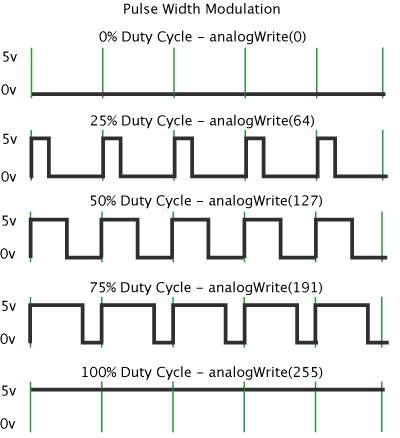
\includegraphics[width=0.45\textwidth]{figs/pwm.png}
\end{center}
\caption{Eight-bit (256) Pulse Width Modulation}
\label{fig:pwm}
\end{figure}

The Arduino Uno has a true analog-to-digital converter (ADC), which
you have already used in the introduction, which can be configured to
read analog inputs on pins A0 through A5.  We'll use interrupt driven
code with a free-running ADC to coax the best performance from the
Arduino.  This will allow us to connect our function generator to a
digital scope.

\begin{figure}[htbp]
\begin{center}
\begin{circuitikz}[line width=1pt]
  \draw (0,0) node[left]{pin $5$ (PWM)} to[short,o-] ++(1.0,0.0)
  to[R,l_=$R$] ++(0,-2) coordinate(X) to[short,-o] ++(-1.0,0.0)
  node[left]{pin $8$ (digital)}; \draw (X) to[short,*-*] ++(0.0,-1)
  coordinate(X) to[short,-o] ++(1.0,0.0) node[right]{pin $A5$
    (scope)}; \draw (X) to[C,l_=$C$] ++(0.0,-2)
  node[ground,yscale=2.0]{};

\end{circuitikz} 
\caption{The PWM output of the function generator at pin 5 is filtered
  by the low-pass $RC$ filter, providing smooth input to the digital
  scope at A5.  Sharp digital features, such as the step function or
  the sharp edge of the sawtooth function, can be applied at pin 8,
  by-passing the filter resistor $R$.}
\label{fig:design}
\end{center}
\end{figure}

An overview of the design for the digital scope and function generator
is shown in Fig.~\ref{fig:design}.  The digital scope is implemented
using the Arduino's built-in ADC connected to analog pin A5.  The
function generator drives the PWM output at pin 5.  This PWM output is
filtered by a low-pass $RC$ filter designed to cut off the
high-frequency PWM cycles, so the voltage at pin A5 is the average
voltage over each PWM cycle.  This is appropriate for smooth functions
such as sine waves.  For functions with sharp features, such as a step
function, the digital pin 8 is used instead, which by-passes the
filter resistor $R$ which would tend filter out these sharp
(high-frequency) features.  When not driving the output, pin 8 is set
to high-impedance in the software (by setting it to be an input).  The
sawtooth function is the most challening to implement, as it uses the
PWM output on pin 5 during the ramp, and then uses pin 8 to create a
sharp transition after the ramp is complete.

The push-button and potentiometer are used to control the mode and
frequency of the function generator.

\section{Setup}

The setup for this lab is straightforward.  You only need to
physically connect digital pin 8 to analog pin A5 on your custom
proto-board, using a section of wire included in your kit.  The
resistor and capacitor are already installed on your proto-board.  In
the Arduino IDE, compile and upload the software from the course
website.  Start the serial plotter at 115200 baud.  Step through wave
form types by pressing the user push-button, and adjust the frequency
with the potentiometer knob.  An example sawtooth waveform is shown in
Fig.~\ref{fig:trace}.

To complete this assignment, take a screenshot of a waveform in your
serial plotter, and submit it to the course website.

\begin{figure}[htbp]
\begin{center}
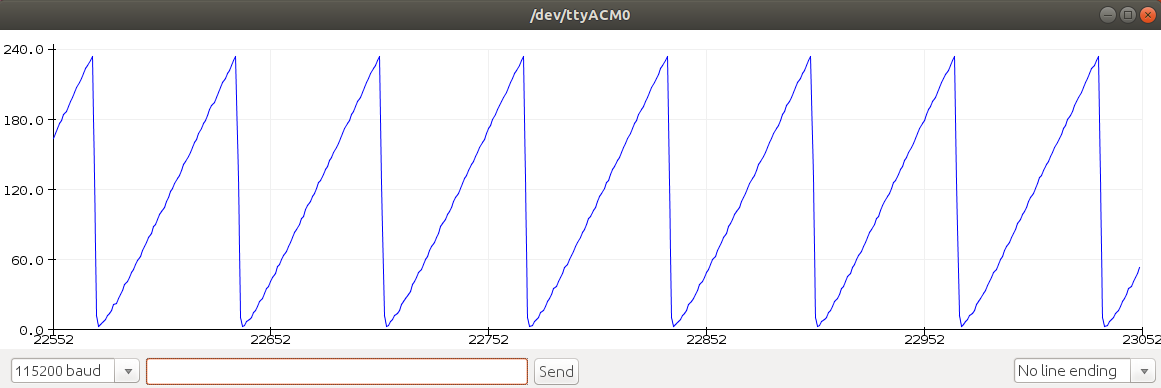
\includegraphics[width=0.95\textwidth]{figs/trace.png}
\end{center}
\caption{Example screen shot of the serial plotter displaying a captured sawtooth function.}
\label{fig:trace}
\end{figure}



\section{Design Improvements}

For fun and extra credit, you can implement a number of design improvements.
\begin{itemize}
\item Adjust the amplitude instead of frequency with the potentiometer.
\item Use the push-button to switch between amplitude or frequency adjustment via potentiometer for each mode.  Use the red LED to indicate which mode you are in.
\item Implement a lock mode (amplitude and frequency locked) which eliminates waveform jitter due to ADC read jitter.
\item This design is quite advanced to get maximum performance from these inexpensive devices.  Start from scratch and implement a much slower, but also much simpler function generator using just analogRead and analogWrite instead of these advanced interrupt driven techniques.
\item Implement a trigger.  This design simply plots the waveform from a random time interval, which is why the phase keeps changing.
\end{itemize}
If you have any other ideas, go ahead and try them.  You can keep your kit over the summer, so have some fun with it.

\end{document}
